\section{Machine Vision}
\subsection{Accuracy of optical distance measurements}
\subsubsection{Experimental setup}
Our experiment consists of two data sets. The first data set is a 2 minute hand-held video footage pointing at the marker that has been measured beforehand at 7 metres away, while the second is a marker at 3 metres away. To illuminate the marker a single 40w incandescent bulb was used at 1.8 metres away from the subject, which yields approximately 14 lux of illuminance. To put it into perspective, a typical library will have an illumination of 500 lux.
\subsubsection{7 metres away}
The distance approximations the program made for the duration of the 2 minute footage was collected for further statistical analysis. Below follows the result.
\begin{verbatim}
Mean:	7.083622663633182
Standard Error:	0.0026907757522701913
Median:	7.09145
Mode:	6.91049
Standard Deviation:	0.1438244181066202
Sample Variance:	0.020685463243707895
Kurtosis:	0.41526910901933745
Skewness:	-0.0038121380062097533
Range:	1.1244000000000005
\end{verbatim}
From the above one can see that the approximations are satisfactory. Below follows the distribution of the readings:\par
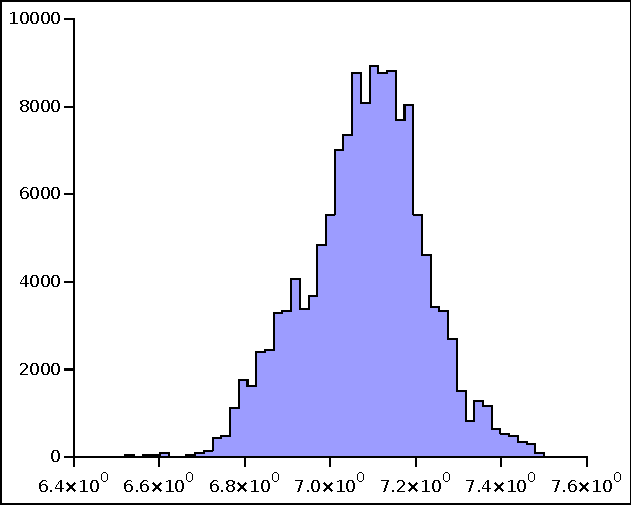
\includegraphics[]{machine_vision/data/7metres.pdf}
\subsubsection{3 metres away}
In the same vein as the above section we obtained the following statistics for 3 metre approximations.
\begin{verbatim}
Mean:	3.1377264426478018
Standard Error:	0.00032314424822403777
Median:	3.13627
Mode:	3.12397
Standard Deviation:	0.020329857058631336
Sample Variance:	0.0004133030880243824
Kurtosis:	-0.5017583141414064
Skewness:	0.20734696083618784
Range:	0.13027999999999995
\end{verbatim}
\par
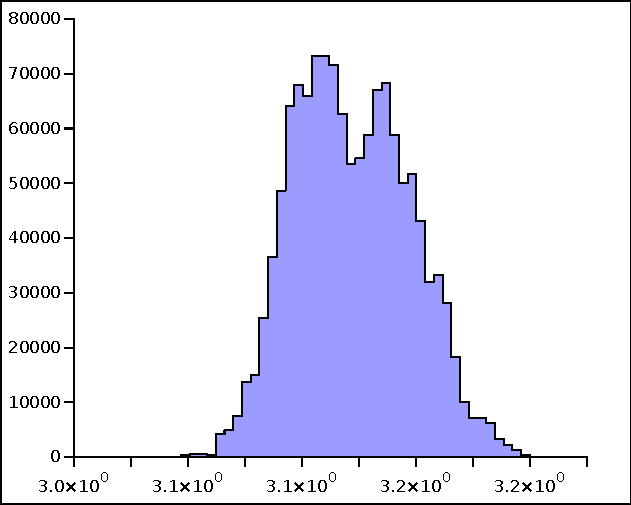
\includegraphics[]{machine_vision/data/3metres.pdf}
\subsection{Other field tests}
On the outdoors test one notices rare and spurious false positive tag identification, specifically tag id 17. There are a number of remediation strategies that one could employ to reduce the likelihood of false positives or even elimitate them entirely for all intents and purposes.
\subsubsection{Double markers}
\subsubsection{Emperical elimination of bad tags}
\subsubsection{Stronger hamming codes}
